\documentclass[11pt]{article}
\usepackage[margin=0.86in]{geometry}
\usepackage{amsmath,amssymb,amsthm,mathtools}
\usepackage{microtype}
\usepackage{booktabs}
\usepackage{enumitem}
\usepackage{tikz}
\usetikzlibrary{arrows.meta,calc,decorations.pathreplacing,positioning}
\usepackage[hidelinks]{hyperref}
\setlist{nosep}
\newtheorem{theorem}{Theorem}[section]
\newtheorem{lemma}[theorem]{Lemma}
\newtheorem{corollary}[theorem]{Corollary}
\newtheorem{proposition}[theorem]{Proposition}
\theoremstyle{definition}
\newtheorem{definition}[theorem]{Definition}
\newtheorem{warning}[theorem]{Warning}
\theoremstyle{remark}
\newtheorem{remark}[theorem]{Remark}
\newcommand{\EL}{\operatorname{EL}}
\newcommand{\Tr}{\operatorname{Tr}}
\newcommand{\op}{\mathrm{op}}
\title{Proposed Manuscript Insertions V\\
The Physical Direct-Decoration Collar and Compact Multi-Port Response}
\author{Research draft for the marked-width MLC program}
\date{July 25, 2026}

\begin{document}
\maketitle

\begin{abstract}
We resolve an actual physical cell $P\setminus Q_a^\circ$, rather than an
ideal equal-footprint rectangle.  The physical set splits into an inactive
common-ray attachment skeleton and an active Jordan quadrilateral.  At an
intermediate puzzle boundary, the outgoing and incoming active footprints are
generally unequal: only their common atoms are glued, both one-sided differences
remain side ports, and the overlap of the inactive attachment arcs remains
nonconducting metadata.  Compatible Douglas trace spaces give exact
fiber-product response composition and functorial last-use elimination.  The
physical shell resistances satisfy a serial lower bound.  Once the finite live
port frontier is frozen, the remaining multi-port response has a compact
operator limit and an explicit accumulated-resistance estimate.  This proves the
direct-decoration trace-collar realization and removes an independent analytic
end-plumbing gap; the universal horizon, H2, MBTT, UPTCR, and MLC remain open.
\end{abstract}

\section{The physical set and its conducting cell}

Let $P$ be the source direct-decoration puzzle piece and let $Q_a\subset P$ be
one of its univalent pullbacks.  The source $Q_a$ is attached to the two boundary
rays of $P$ landing at one vertex.  Their common ray portions form a closed arc
$A_a\subset\partial P\cap\partial Q_a$, with endpoints $x_a^-,x_a^+$.
Let $y_a^\pm$ be the parent equipotential endpoints and define the parent
footprint $\Gamma_a^-$, child footprint $\Gamma_a^+$, and exposed ray sides
$S_a^\pm$ as in Figure~\ref{fig:physical-cell}.

\begin{figure}[htbp]
\centering
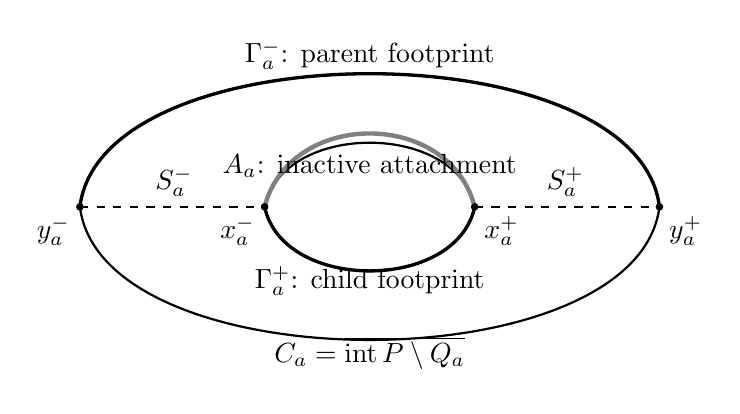
\begin{tikzpicture}[scale=0.92,>=Latex]
  \draw[thick] (-4,0) .. controls (-3.7,2.45) and (3.7,2.45) .. (4,0)
               .. controls (3.7,-2.45) and (-3.7,-2.45) .. cycle;
  \draw[thick] (-1.45,0) .. controls (-1.2,1.18) and (1.2,1.18) .. (1.45,0)
               .. controls (1.2,-1.18) and (-1.2,-1.18) .. cycle;
  \draw[very thick] (-4,0) .. controls (-3.7,2.45) and (3.7,2.45) .. (4,0);
  \draw[very thick] (-1.45,0) .. controls (-1.2,-1.18) and (1.2,-1.18) .. (1.45,0);
  \draw[dashed,thick] (-4,0)--(-1.45,0);
  \draw[dashed,thick] (1.45,0)--(4,0);
  \draw[ultra thick,gray] (-1.45,0) .. controls (-1.1,1.35) and (1.1,1.35) .. (1.45,0);
  \node at (0,2.1) {$\Gamma_a^-$: parent footprint};
  \node at (0,-1.02) {$\Gamma_a^+$: child footprint};
  \node at (-2.7,0.34) {$S_a^-$};
  \node at (2.7,0.34) {$S_a^+$};
  \node at (0,0.57) {$A_a$: inactive attachment};
  \node at (0,-2.02) {$C_a=\overline{\operatorname{int}P\setminus Q_a}$};
  \fill (-1.45,0) circle (1.5pt) node[below left] {$x_a^-$};
  \fill (1.45,0) circle (1.5pt) node[below right] {$x_a^+$};
  \fill (-4,0) circle (1.5pt) node[below left] {$y_a^-$};
  \fill (4,0) circle (1.5pt) node[below right] {$y_a^+$};
\end{tikzpicture}
\caption{The physical set contains the active quadrilateral $C_a$ and the
inactive common-ray attachment $A_a$.  Additional protected or response ports
are retained as subarcs of the active boundary.}
\label{fig:physical-cell}
\end{figure}

Put
\[
 \Omega_a=\operatorname{int}P\setminus Q_a,
 \qquad C_a=\overline{\Omega_a}.
\]

\begin{theorem}[Active/inactive decomposition]
For nested Jordan disks with common attachment arc $A_a$,
\[
 \boxed{P\setminus Q_a^\circ=C_a\cup A_a,
 \qquad C_a\cap A_a=\{x_a^-,x_a^+\}.}
 \tag{1.1}
\]
The set $C_a$ is a closed Jordan disk with cyclic boundary
\[
 \Gamma_a^-,\quad S_a^+,\quad\Gamma_a^+,\quad S_a^-.
 \tag{1.2}
\]
The relative interior of $A_a$ is not approached from $\Omega_a$ and therefore
carries no independent Dirichlet-to-Neumann trace of the active cell.  It is
retained as attachment/access metadata.
\end{theorem}

\begin{proof}
At an interior point of a common boundary arc, nested Jordan disks lie on the
same side and their interiors agree locally.  Hence the conducting complement
does not approach the relative interior of $A_a$.  Removing $A_a^\circ$ from
$\partial P$ leaves $S_a^-\cup\Gamma_a^-\cup S_a^+$, while removing it from
$\partial Q_a$ leaves $\Gamma_a^+$.  The two residual arcs meet only at
$x_a^\pm$ and form the Jordan curve bounding $C_a$.  This also gives (1.1).
\end{proof}

Consequently there is a prime-end conformal map
\[
 \Psi_a:C_a^\circ\longrightarrow(0,R_a)\times(0,1)
\]
sending the footprints to the vertical sides, where
\[
 R_a=\EL_{C_a}(\Gamma_a^-,\Gamma_a^+)>0.
 \tag{1.3}
\]
No Euclidean-length or trace-density equality is asserted.  For a word $w$,
$C_{w,a}=\phi_w(C_a)$ has the same modulus and transported marked traces.

If extra boundary contacts occur, overlay the two finite ray/equipotential
boundary graphs, subdivide at all vertices, and add finitely many paired
crosscuts to make Jordan cells.  Exact trace gluing below removes the artificial
cuts and recovers the original response.

\section{Unequal successive footprints}

At an intermediate cylinder $Q=Q_{wa}$, let $A^-$ be the inactive attachment
inherited from the preceding cell and $A^+$ the inactive attachment of the next
child.  The active footprints are
\[
 F^{\rm out}=\overline{\partial Q\setminus A^-},
 \qquad
 F^{\rm in}=\overline{\partial Q\setminus A^+}.
 \tag{2.1}
\]
Subdivide at all attachment and proof-use endpoints.  The relatively open atoms
have the exact classification
\[
\begin{aligned}
 I&=\partial Q\setminus(A^-\cup A^+) &&\text{common active glue},\\
 E^{\rm out}&=A^+\setminus A^- &&\text{outgoing-only side port},\\
 E^{\rm in}&=A^-\setminus A^+ &&\text{incoming-only side port},\\
 Z&=A^-\cap A^+ &&\text{double-inactive attachment}.
\end{aligned}
\tag{2.2}
\]
Endpoints form a finite fifth class $V$.  Only $I$ is glued; $E^{\rm out}$ and
$E^{\rm in}$ remain physical boundary ports; $Z$ is marked but nonconducting.

\begin{figure}[htbp]
\centering
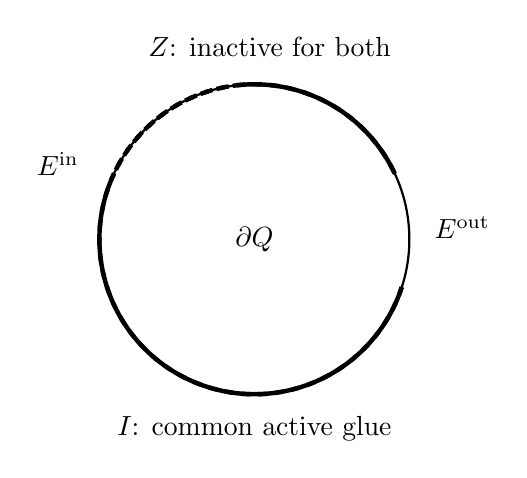
\begin{tikzpicture}[scale=0.96]
  \draw[thick] (0,0) circle (2.05);
  \draw[ultra thick] (155:2.05) arc (155:342:2.05);
  \draw[ultra thick,dashed] (342:2.05) arc (342:25:2.05);
  \draw[ultra thick] (25:2.05) arc (25:95:2.05);
  \draw[ultra thick,dashed] (95:2.05) arc (95:155:2.05);
  \node at (0,-2.5) {$I$: common active glue};
  \node at (2.75,0.15) {$E^{\rm out}$};
  \node at (-2.6,1.0) {$E^{\rm in}$};
  \node at (0.2,2.55) {$Z$: inactive for both};
  \node at (0,0) {$\partial Q$};
\end{tikzpicture}
\caption{Schematic common refinement.  Solid arcs are active from at least one
cell; dashed arcs indicate attachment intervals.  Actual endpoints are supplied
by the puzzle rays and every declared proof-use port.}
\label{fig:refinement}
\end{figure}

Freeze a finite proof horizon and insert endpoints of every footprint,
intersection, protected collar, obstacle interface, response electrode, ideal
interval, and authorized presentation map.  The resulting finite trace atoms
transport exactly under every inverse word.  If the source boundary starts with
$N_\partial$ atoms and $m$ marked subarcs are added, there are at most
$N_\partial+2m$ relatively open atoms after duplicate endpoints are removed.
Two connected attachment arcs have at most four distinct endpoints, so each
ordered symbol pair has at most four open atoms and four endpoint atoms.  For an
alphabet of size $d$, the unmarked structural atlas therefore has at most
$8d^2$ local types, independently of depth.  Any one-sided atom not seeded by a
future observable is eliminated at its birth junction by (3.5).

\section{Compatible trace spaces and exact composition}

A naive direct sum of $H^{1/2}$ spaces on adjacent arcs can lose endpoint
compatibility.  For a marked Jordan cell $\Omega$ and a finite active boundary
union $G$, use the actual quotient trace space
\[
 \mathcal T_\Omega(G)=\{\Tr_Gu:u\in H^1(\Omega)\}
 \tag{3.1}
\]
with its quotient norm.  Equivalently, use the Douglas trace space on the
prime-end circle and restrict to $G$.  Define
\[
 q_{\Omega,G}(\tau)=
 \inf_{\Tr_Gu=\tau}\int_\Omega|\nabla u|^2.
 \tag{3.2}
\]
Unlisted active boundary is natural Neumann boundary.

\begin{theorem}[Fiber-product response composition]
Let two active cells have disjoint interiors and common active trace $I$.  Let
$r_i$ be restriction to $I$ and let $e_i$ retain every other live trace label.
Then the response of the physical union is
\[
 \boxed{
 q(x_1,x_2)=\inf
 \left\{q_1(\tau_1)+q_2(\tau_2):
 r_1\tau_1=r_2\tau_2,\ e_i\tau_i=x_i\right\}.}
 \tag{3.3}
\]
The one-sided atoms remain among $x_1,x_2$.  Composition is associative and
conformally natural.
\end{theorem}

\begin{proof}
Restriction of a finite-energy function gives matching common traces and
additive energy.  Conversely, two finite-energy functions with matching trace
glue to a finite-energy function on the union.  The quotient trace spaces retain
all endpoint compatibility.  Joint infima are independent of elimination order.
\end{proof}

For a continuous forgetful map $p:T\to T_{\rm live}$, put
\[
 (p_*q)(y)=\inf_{p\tau=y}q(\tau).
 \tag{3.4}
\]

\begin{theorem}[Functorial last-use elimination]
For composable forgetful maps,
\[
 (r\circ p)_*q=r_*(p_*q).
 \tag{3.5}
\]
Hence a side port may be deleted exactly at its last proof use, even when its
trace is endpoint-compatible with neighboring atoms.
\end{theorem}

If at most $b$ ports are born per stage and every port has future lifetime at
most $L$, the live non-interface frontier has size at most $b(L+1)$.

\section{Accumulated physical resistance}

For $w=a_1\cdots a_m$, let
\[
 C_j=\overline{\operatorname{int}Q_{a_1\cdots a_{j-1}}
 \setminus Q_{a_1\cdots a_j}},
 \qquad R_j=R_{a_j}.
\]
Every complete outer-to-terminal curve crosses the conducting cells in
chronological order.

\begin{theorem}[Extremal series lower bound]
The selected physical tail resistance satisfies
\[
 \boxed{R(w)\ge\sum_{j=1}^mR_{a_j}.}
 \tag{4.1}
\]
For a finite root-cell alphabet,
\[
 R_*:=\min_aR_a>0,
 \qquad R(w)\ge mR_*.
 \tag{4.2}
\]
\end{theorem}

\begin{proof}
Choose almost extremal metrics $\rho_j$ supported in the disjoint conducting
cells, normalized so each cell crossing has length at least one and area close
to $1/R_j$.  The metric $\sum c_j\rho_j$ gives every complete crossing length
at least $\sum c_j$ and area close to $\sum c_j^2/R_j$.  Taking $c_j=R_j$
gives (4.1).
\end{proof}

A later wiring that identifies side ports from separated levels may create a
bypass and must be included before (4.1) is invoked.

\section{Compact multi-port tail response}

Freeze the proof-use inventory, eliminate every dead port by (3.5), and choose a
stage after the last live non-interface side port.  The unequal-footprint prefix
is one exact compatible form $q_{\rm L}$ on $X\times\mathcal H_{\rm in}$; let
$q_{\rm R}$ be the terminal cap form on $\mathcal H_{\rm out}\times Y$.
Compose every remaining physical shell exactly by (3.3).  The selected conducting
component uniformizes, after any finite overlay cuts are recomposed, to a strip or
cylinder of resistance
\[
 R\ge\sum_{j>N}R_{a_j}.
 \tag{5.1}
\]
Let $A$ be its tangential operator, with kernel the constants and first positive
eigenvalue $\lambda_1>0$ ($\lambda_1=\pi$ for the width-one Neumann strip).
The complete response is
\[
 q_R(x,y)=\inf_{\phi,\psi}
 \left[q_{\rm L}(x,\phi)+\mathcal N_R(\phi,\psi)
 +q_{\rm R}(\psi,y)\right].
 \tag{5.2}
\]

Let $\mathcal N_R^\#$ retain the exact scalar resistor $1/R$ and the two
mean-zero half-cylinder responses.  With
\[
 \eta_A(R)=\frac{2}{e^{\lambda_1R}-1},
\]
\[
 (1-\eta_A(R))q_R^\#\preceq q_R
 \preceq(1+\eta_A(R))q_R^\#.
 \tag{5.3}
\]
Define the half-cylinder-closed cap forms
\[
 \widehat q_{\rm L}(x,c)=\inf_{\xi\perp\mathbf1}
 \left[q_{\rm L}(x,c\mathbf1+\xi)+\langle A\xi,\xi\rangle\right],
\]
\[
 \widehat q_{\rm R}(d,y)=\inf_{\zeta\perp\mathbf1}
 \left[q_{\rm R}(d\mathbf1+\zeta,y)+\langle A\zeta,\zeta\rangle\right].
\]
Then exactly
\[
 q_R^\#(x,y)=\inf_{c,d\in\mathbb C}
 \left[\widehat q_{\rm L}(x,c)+\frac{|c-d|^2}{R}
 +\widehat q_{\rm R}(d,y)\right].
 \tag{5.4}
\]

Write, modulo the global constant,
\[
 \widehat q_{\rm L}(x,c)=\langle Lx,x\rangle
 +2\Re\langle b_{\rm L}x,c\rangle+\alpha_{\rm L}|c|^2
\]
and similarly on the right.  Positivity gives
$\alpha_i=0\Rightarrow b_i=0$.

\begin{theorem}[Compact multi-port response]
For a fixed physical prefix and terminal cap, or for the finitely many types in a
frozen branch graph, $q_R$ extends continuously to $R=\infty$ in normalized
response-operator norm.  Its parameter image is compact.  If
$\alpha_{\rm L},\alpha_{\rm R}>0$, set
$\alpha_*=\min(\alpha_{\rm L},\alpha_{\rm R})$.  If $B$ bounds the
external-to-scalar coupling and $M$ bounds $\|q_R^\#\|$, then
\[
 \boxed{
 \|q_R-q_\infty\|
 \le M\frac{2}{e^{\lambda_1R}-1}
 +\frac{2B^2}{\alpha_*^2R}.}
 \tag{5.5}
\]
If either scalar cap coefficient is zero, the second term is exactly absent.
\end{theorem}

\begin{proof}
The internal scalar matrix is
\[
 M_t=\begin{pmatrix}\alpha_{\rm L}+t&-t\\-t&\alpha_{\rm R}+t\end{pmatrix},
 \qquad t=R^{-1}.
\]
When both coefficients are positive, the resolvent identity gives
$\|M_t^{-1}-M_0^{-1}\|\le2t/\alpha_*^2$, and the scalar Schur complement changes
by at most $2B^2/(\alpha_*^2R)$.  If one coefficient vanishes, its coupling
vanishes by positivity and direct inversion shows that the visible scalar Schur
complement is independent of $t$.  Equation (5.3) contributes at most
$2M/(e^{\lambda_1R}-1)$.  This proves (5.5) and norm continuity.
\end{proof}

For response error at most $\varepsilon$, it is sufficient that
\[
 \boxed{
 R\ge\max\left\{
 \frac1{\lambda_1}\log\left(1+\frac{4M}{\varepsilon}\right),
 \frac{4B^2}{\alpha_*^2\varepsilon}
 \right\}.}
 \tag{5.6}
\]
Omit the second term in the zero-coefficient cases.  A sufficient additional
physical depth is the ceiling of the right side divided by $R_*$.

\section{Gate decisions}

\begin{theorem}[Physical direct-decoration trace-collar realization]
Every source direct-decoration $P\setminus Q_a^\circ$ has an exact finite
active/inactive ray/equipotential decomposition.  Actual unequal footprints,
one-sided side ports, double-inactive attachment arcs, protected intervals,
obstacles, and response electrodes are retained by the common-refinement atlas;
composition and artificial-cut removal are exact; and the complete construction
transports under every finite inverse word.  Thus
\[
 \boxed{\texttt{DIRECT\_DECORATION\_TRACE\_COLLAR\_REALIZATION}}
\]
is proved in the source direct-decoration category.
\end{theorem}

\begin{theorem}[Corrected end-plumbing trace response]
Once the upstream finite inventory supplies a last live non-interface side-port
stage, the physical tail has an exact fixed multi-port prefix, exact full-trace
tail response, exact last-use elimination, compact operator limit, and the
explicit estimates (5.5)--(5.6).  Therefore
\[
 \boxed{\texttt{END\_PLUMBING\_TRACE\_RESPONSE\_CONTROL}}
\]
has no remaining independent analytic gap; its remaining dependency is the
finite live frontier supplied by \texttt{VAAPC-I} or the horizon theorem.
\end{theorem}

For an already supplied direct-decoration branch graph of depth $H$, the
unmarked structural transition atlas has at most $8d^2$ local types and every
unseeded one-sided atom is immediately eliminated.  With $N_0$ root trace atoms
and alphabet size $d$, the full raw pullback atlas has at most
\[
 N_0\sum_{j=0}^{H}d^j
\]
records before dependency closure.  This proves the direct-decoration trace
portion of frozen input.  Global \texttt{VAAPC-I} remains open because the
source-faithful complete Wave demand graph and final horizon are not yet known.

\section{Failure record and remaining path}

A failed application must name the first extra contact, inaccessible attachment
inserted as a conducting trace, missing refinement endpoint, false glue atom,
discarded one-sided side port, electrically misclassified double-inactive atom,
phase or endpoint-compatibility defect, side-port bypass, infinite live frontier,
zero modulus, failed cap normalization, or insufficient accumulated resistance.

This result does not prove the universal Wave horizon, global \texttt{VAAPC-I},
the common primitive, neutral, and virtual response and Value calibration
required by H2, the root contraction and discounted error budget required by MBTT,
coercivity, rigidity, UPTCR, or MLC.  The next response theorem is a universal
bounded-lifetime law or future-faithful quotient for the live common-refinement
port frontier, followed by uniform comparison with the KKL WAD/Value and neutral
sectorial charts.

\end{document}
